\chapter{Základné pojmy}



%%%%%%%%%%%%%%%%%%%%%%%%%%%%%%%%%%%%%%%%%%%%%%%%%%%%%%%%%%%%%%%%%%%%%%%%%%%%%%%%%%%%%%%%%%%%%%%%%%%%%%%%%%%%%%%%%%%%%%%%%%%%%%%%%%%%%%%%%%%%%%%%%%%%%%%%%%%%%%%%%%%%%%%%%%%%%%%%%%%%%%%%%%%%%%%%%%%%%%%%%%%%%%%%%%%%%%%%%%%%%%%%%%%%%%%%%%%%%%%%%%%%%%%%%

\section{HTML 5 štandardy}

\ac*{HTML} 

http://www.w3.org/TR/html5/  

The World Wide Web's markup language has always been HTML. HTML was primarily designed as a language for semantically describing scientific documents, although its general design and adaptations over the years have enabled it to be used to describe a number of other types of documents.

The main area that has not been adequately addressed by HTML is a vague subject referred to as Web Applications. This specification attempts to rectify this, while at the same time updating the HTML specifications to address issues raised in the past few years.

1.2 Audience

This section is non-normative.

This specification is intended for authors of documents and scripts that use the features defined in this specification, implementors of tools that operate on pages that use the features defined in this specification, and individuals wishing to establish the correctness of documents or implementations with respect to the requirements of this specification.

This document is probably not suited to readers who do not already have at least a passing familiarity with Web technologies, as in places it sacrifices clarity for precision, and brevity for completeness. More approachable tutorials and authoring guides can provide a gentler introduction to the topic.

In particular, familiarity with the basics of DOM is necessary for a complete understanding of some of the more technical parts of this specification. An understanding of Web IDL, HTTP, XML, Unicode, character encodings, JavaScript, and CSS will also be helpful in places but is not essential.

1.3 Scope

This section is non-normative.

This specification is limited to providing a semantic-level markup language and associated semantic-level scripting APIs for authoring accessible pages on the Web ranging from static documents to dynamic applications.

The scope of this specification does not include providing mechanisms for media-specific customization of presentation (although default rendering rules for Web browsers are included at the end of this specification, and several mechanisms for hooking into CSS are provided as part of the language).

The scope of this specification is not to describe an entire operating system. In particular, hardware configuration software, image manipulation tools, and applications that users would be expected to use with high-end workstations on a daily basis are out of scope. In terms of applications, this specification is targeted specifically at applications that would be expected to be used by users on an occasional basis, or regularly but from disparate locations, with low CPU requirements. Examples of such applications include online purchasing systems, searching systems, games (especially multiplayer online games), public telephone books or address books, communications software (e-mail clients, instant messaging clients, discussion software), document editing software, etc.

1.4 History



blal 3.2.5.1 The id attribute

The id attribute specifies its element's unique identifier (ID). [DOM]

The value must be unique amongst all the IDs in the element's home subtree and must contain at least one character. The value must not contain any space characters.





\section{Čo je SVG?}
\ac{SVG} je štandardný formát pre vektorovú grafiku. Vektorová grafika je definovaná cez body, priamky, mnohouholníky, elipsy, krivky, alebo iné geometrické tvary.  

\acs{SVG} je aplikácia \ac*{XML}, ktorá umožňuje reprezentáciu grafických informácii v kompaktnom, prenositeľnom tvare. 

Prispôsobiteľnosť SVG umožňuje zmeniť veľkosť grafického komponentu bez straty kvality vzhľadu. Čo umožňuje zobraziť responzívne na viacerých možných zariadení. 
SVG sa bude zobrazovať rovnako na rôznych platformách. Je kompatibilná s štandardmi \acs{HTML}5, ktoré navrhla \ac*{W3C}.  


http://www.w3.org/Graphics/SVG/About.html

SVG is a language for describing two-dimensional graphics in XML. SVG allows for three types of graphic objects: vector graphic shapes (e.g., paths consisting of straight lines and curves), images and text. Graphical objects can be grouped, styled, transformed and composited into previously rendered objects. Text can be in any XML namespace suitable to the application, which enhances searchability and accessibility of the SVG graphics. The feature set includes nested transformations, clipping paths, alpha masks, filter effects, template objects and extensibility.

SVG drawings can be dynamic and interactive. The Document Object Model (DOM) for SVG, which includes the full XML DOM, allows for straightforward and efficient vector graphics animation via scripting. A rich set of event handlers such as onmouseover and onclick can be assigned to any SVG graphical object. Because of its compatibility and leveraging of other Web standards, features like scripting can be done on SVG elements and other XML elements from different namespaces simultaneously within the same Web page.
 
 
 \section{Browser Support}
 The numbers in the table specify the first browser version that fully supports the $<$svg$>$ element.
 Element					
 $<$svg$>$	4.0	9.0	3.0	3.2	10.1
 \subsection{Differences Between SVG and Canvas}
 SVG is a language for describing 2D graphics in XML.
 Canvas draws 2D graphics, on the fly (with a JavaScript).
 SVG is XML based, which means that every element is available within the SVG DOM. You can attach JavaScript event handlers for an element.
 In SVG, each drawn shape is remembered as an object. If attributes of an SVG object are changed, the browser can automatically re-render the shape.
 Canvas is rendered pixel by pixel. In canvas, once the graphic is drawn, it is forgotten by the browser. If its position should be changed, the entire scene needs to be redrawn, including any objects that might have been covered by the graphic.
 
 
 \subsection{Comparison of Canvas and SVG}
 The table below shows some important differences between Canvas and SVG:
 Canvas
 
 \begin{enumerate}
 	\item	Resolution dependent
 	\item	No support for event handlers
 	\item	Poor text rendering capabilities
 	\item	You can save the resulting image as .png or .jpg
 	\item	Well suited for graphic-intensive games
 \end{enumerate}	
 SVG
 
 \begin{enumerate}
 	\item	Resolution independent
 	\item	Support for event handlers
 	\item	Best suited for applications with large rendering areas (Google Maps)
 	\item	Slow rendering if complex (anything that uses the DOM a lot will be slow)
 	\item	Not suited for game applications
 \end{enumerate}
 
 
 
 
 \section{Základná syntax \acs*{SVG}}

V HTML5 sa môžu používať vložené SVG elementy priamo v na HTML stránke. 

\subsection{Príklad jednoduchého SVG komponentu}

HTML kód: 

\begin{lstlisting}
<!DOCTYPE html>
<html>
<head lang="sk">
<meta charset="UTF-8">
<title></title>
</head>
<body>

	<svg width="100" height="100">
		<circle cx="50" cy="50" r="40" stroke="black" stroke-width="2" fill="silver" />
	</svg>	
	
</body>
</html>

\end{lstlisting}


\subsubsection{Vysvetlenie SVG kódu}

Každý SVG obrázok začína s $<$svg$>$ elementom. Atribúty elementu $<$svg$>$ sú width a height. Definujú šírku a výšku SVG obrázka. Element $<$circle$>$ je použitý na nakreslenie kruhu. Atribúty cx, cy definujú x, y súradnice od centra kruhu. Ak je cx, cy vynechané, tak center kruhu je nastavený na $($0, 0$)$. Atribút r  definuje polomer kruhu. Atribúty stroke a stroke=width určujú to ako bude vyzerať obrys útvaru. Nastavila som 2px čierny okraj. 
Atribút fill vyplní vnútro kruhu. V príklade sa mi vyplnilo sivou farbou. Tag, ktorý uzavrie SVG obrázok je $<$$/$svg$>$. Keďže SVG je napísané XML, tak všetky elementy musia byť správne zatvorené. 
%zdroj www.w3schools.com/svg/svg_inhtml.asp


Vykreslí na HTML stránku útvar, ktorý je na obrázku \ref{jednoduchyKruh}.

\begin{figure}[ht]
	\begin{center}
		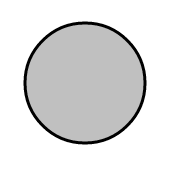
\includegraphics  {obrazky/jednoduchyKruh.png}
		\caption{Vykreslenie SVG na HTML stránke}
		\label{jednoduchyKruh}
	\end{center}
\end{figure}


\section{SVG útvary} 

\acs*{SVG} má preddefinované tieto tvary elementov:
\begin{itemize}
	\item Obdĺžník $<$rect$>$
	\item Kruh $<$circle$>$
	\item Elipsa $<$ellipse$>$
	\item Čiara $<$line$>$
	\item Polyline $<$polyline$>$
	\item Mnohouholník $<$polygon$>$
	\item Cesta $<$path$>$	
\end{itemize}

\section{CSS vlastnosti}

Podľa HTML5 štandardov dokáže CSS meniť vlastnosti SVG.

%www.w3.org/tr/svg/styling.html
%http://www.w3.org/TR/SVG/propidx.html http://www.w3.org/TR/SVG2/styling.html

Vymenované vlastnosti, ktoré majú rovnaké \acs{CSS} 2.1 a \acs{SVG}. Z toho vyplýva, že SVG vlastnosti môžem meniť aj cez CSS selektor. 

Vlastnosti písma:
\begin{itemize}
	\item 	‘font’ - písmo
	\item 	‘font-family’ - rodinu písiem
	\item 	‘font-size’ - veľkosť písma
	\item 	‘font-style’ - štýl písma
	\item 	‘font-variant’ - varianta písma
\end{itemize}

Vlastnosti textu: 
\begin{itemize}
\item 	‘direction’ - smer
\item 	‘letter-spacing’ 
\item 	‘text-decoration’
\item 	‘unicode-bidi’
\item 	‘word-spacing’
\end{itemize}

Other properties for visual media:
‘clip’, only applicable to outermost svg element.
‘color’, used to provide a potential indirect value (currentColor) for the ‘fill’, ‘stroke’, ‘stop-color’, ‘flood-color’ and ‘lighting-color’ properties. (The SVG properties which support color allow a color specification which is extended from CSS 2.1 to accommodate color definitions in arbitrary color spaces. See Color profile descriptions.)
‘cursor’
‘display’
‘overflow’, only applicable to elements which establish a new viewport.
‘visibility’
The following SVG properties are not defined in CSS 2.1. The complete normative definitions for these properties are found in this specification:
Clipping, Masking and Compositing properties:
‘clip-path’
‘clip-rule’
‘mask’
‘opacity’
Filter Effects properties:
‘enable-background’
‘filter’
‘flood-color’
‘flood-opacity’
‘lighting-color’
Gradient properties:
‘stop-color’
‘stop-opacity’
Interactivity properties:
‘pointer-events’
Color and Painting properties:
‘color-interpolation’
‘color-rendering’
‘fill’
‘fill-opacity’
‘fill-rule’
‘image-rendering’
‘marker’
‘marker-end’
‘marker-mid’
‘marker-start’
‘shape-rendering’
‘stroke’
‘stroke-dasharray’
‘stroke-dashoffset’
‘stroke-linecap’
‘stroke-linejoin’
‘stroke-miterlimit’
‘stroke-opacity’
‘stroke-width’
‘text-rendering’
Text properties:
‘alignment-baseline’
‘baseline-shift’
‘dominant-baseline’
‘glyph-orientation-horizontal’
‘glyph-orientation-vertical’
‘text-anchor’
‘writing-mode’
 


